
\section{System Architectures}

%This section presents the general architectures of the systems we used for the development and experiments in our research. We illustrate the Extraction, Transformation, and Load (ETL) pipeline we used for the medical research papers. Additionally, we have our misinformation classification process, where we classify the health misinformation and refute it. Finally, we have the system's User Interface (UI).

\subsection{Research Paper ETL Pipeline}

Our model must use credible sources of information to rebut misinformation. We identified PubMed \cite{pubmed}, an online library that contains peer-reviewed medical literature. We want to extract the papers and store them in a vector database. To extract these papers, we used the BioC API \cite{bioinformatics}, which has access to the PubMed library. However, the API needs the research paper's identifier, known as PubMed Central (PMC) ID. We design a scraper to extract these identifiers from the official PubMed site. The pipeline in Figure \ref{fig:etl} shows the processes of data extraction. 

\begin{figure}[htbp]
	\begin{center}
		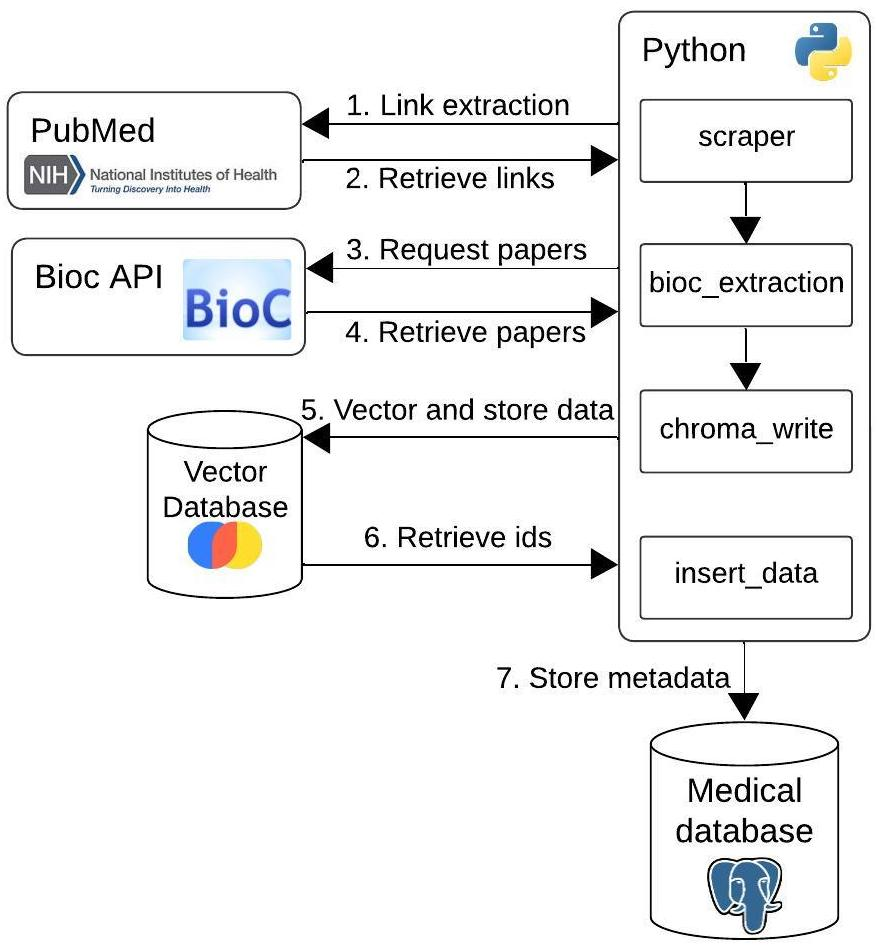
\includegraphics[width=0.4\textwidth]{figures/ETL_Pipeline.jpeg} %specify width
	\end{center}
	\caption{Medical Data Extraction Pipeline} %specify caption
	\label{fig:etl}
\end{figure}

\subsubsection{Scraper}
The first step of the pipeline was identifying what papers we needed to extract. We selected topics based on the datasets we used, some topics were \textit{allergy}, \textit{covid}, \textit{monkeypox}, \textit{zika}, \textit{vaccine}, and others. To extract them, we built a scraper in Python using Selenium and BeautifulSoup libraries. They were used to get the links for each paper. Each link contains the PMC ID and we extracted 5,000 identifiers for each topic.

\subsubsection{BioC API}
Using the PubMed API, BioC, we made requests with the PMC that returned the documents as JSON. Later, the paper's sections -introduction, methodology, results, and others- were combined as one attribute, excluding references. We removed tables, figures, and references from the context to ensure the chunking process worked appropriately. After that, we stored the result into a new JSON that contains the paper's metadata and context. 

\subsubsection{Vectorizing data}
After retrieving the data, we vectorize the papers, Figure \ref{fig:vector} shows this process. First, each research paper’s context was split into chunks using LangChain. Then, we used an LLM, BAAI \cite{bge_embedding}, to embed these chunks. A universal unique identifier (UUID) is combined with each chunk and stored in a Chroma database. After storing the embedding, we added these UUIDs to their JSON. 

\begin{figure}[h]
	\begin{center}
		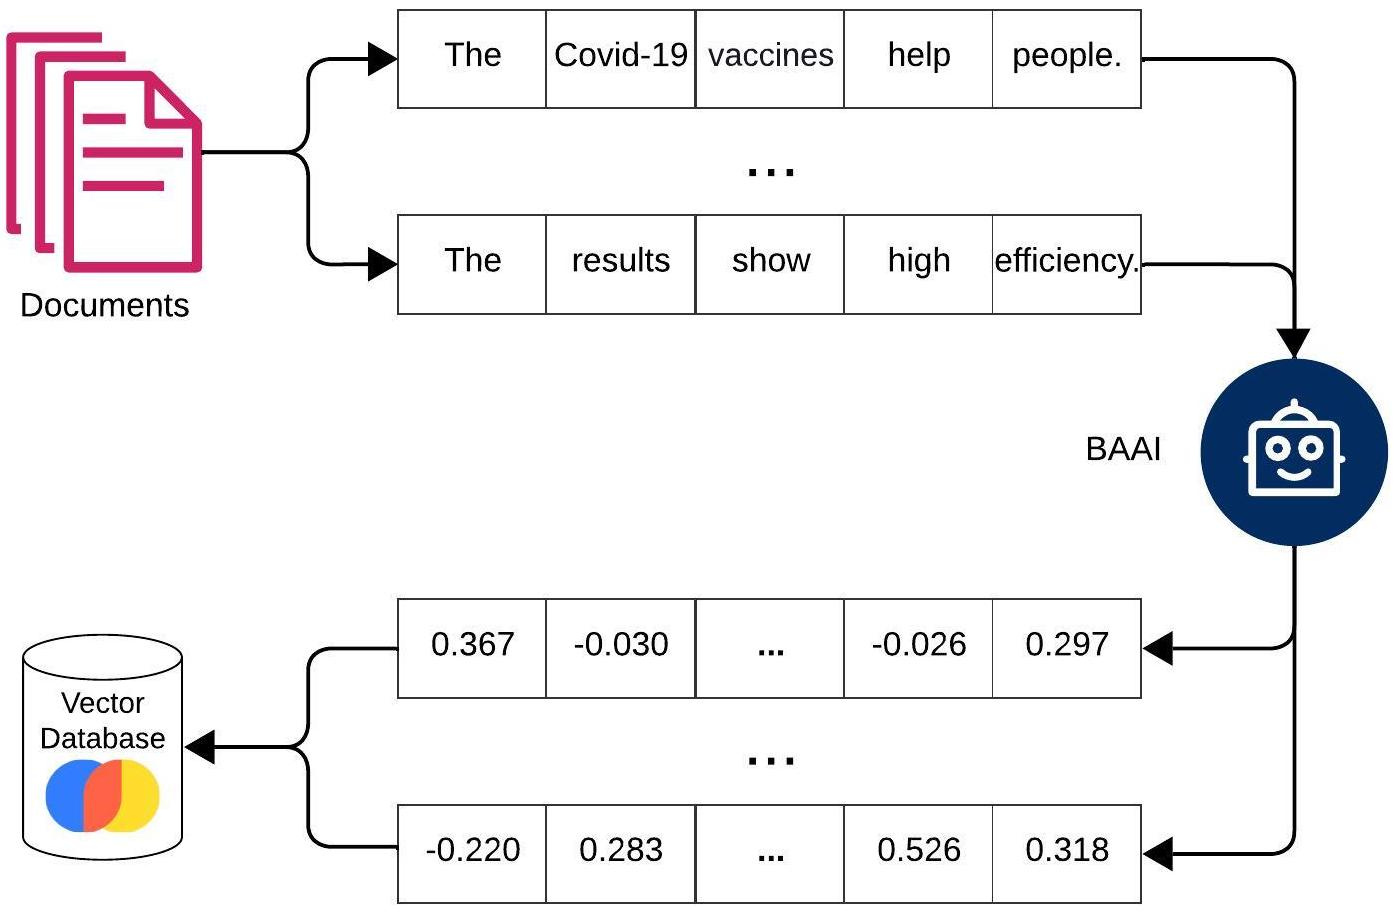
\includegraphics[width=0.42\textwidth]{figures/Data_vectorization.jpeg} %specify width
	\end{center}
	\caption{Data Vectorization Process} %specify caption
	\label{fig:vector}
\end{figure}


\subsubsection{Store metadata}
Now, with all papers vectorized, we upload the metadata into a Postgres database. Duplicates or any research that did not contain at least an abstract were removed. That ensures that there is no repetition or inconsistency when doing the rebuttal. Later, we upload the data into the database following the schema found in Figure \ref{fig:table}. The tables in this schema are as follow:

\begin{description}
	\item{\textbf{Research:}}  Contains the research paper's metadata. Its attributes are: \textit{title}, paper's title; \textit{context}, the paper’s text; \textit{paper\_ref}, the reference of the paper; and \textit{fullpaper}, a boolean that is true if the paper contains an abstract, introduction, methodology, discussion, conclusion, and references.
	\item{\textbf{Chunks:}} Pairs the UUIDs from the paper's chunks and their respective research record.  
	\item{\textbf{Keyword:}} Keywords that allow the reader to know the subjects mentioned in the paper. 
	\item{\textbf{Author:}} Full name of the paper's authors. 
	\item{\textbf{Reference:}} All references present in the paper.
	\item{\textbf{Topic:}} The topics used to search the papers.

\end{description}

\begin{figure}[htbp]
	\begin{center}
		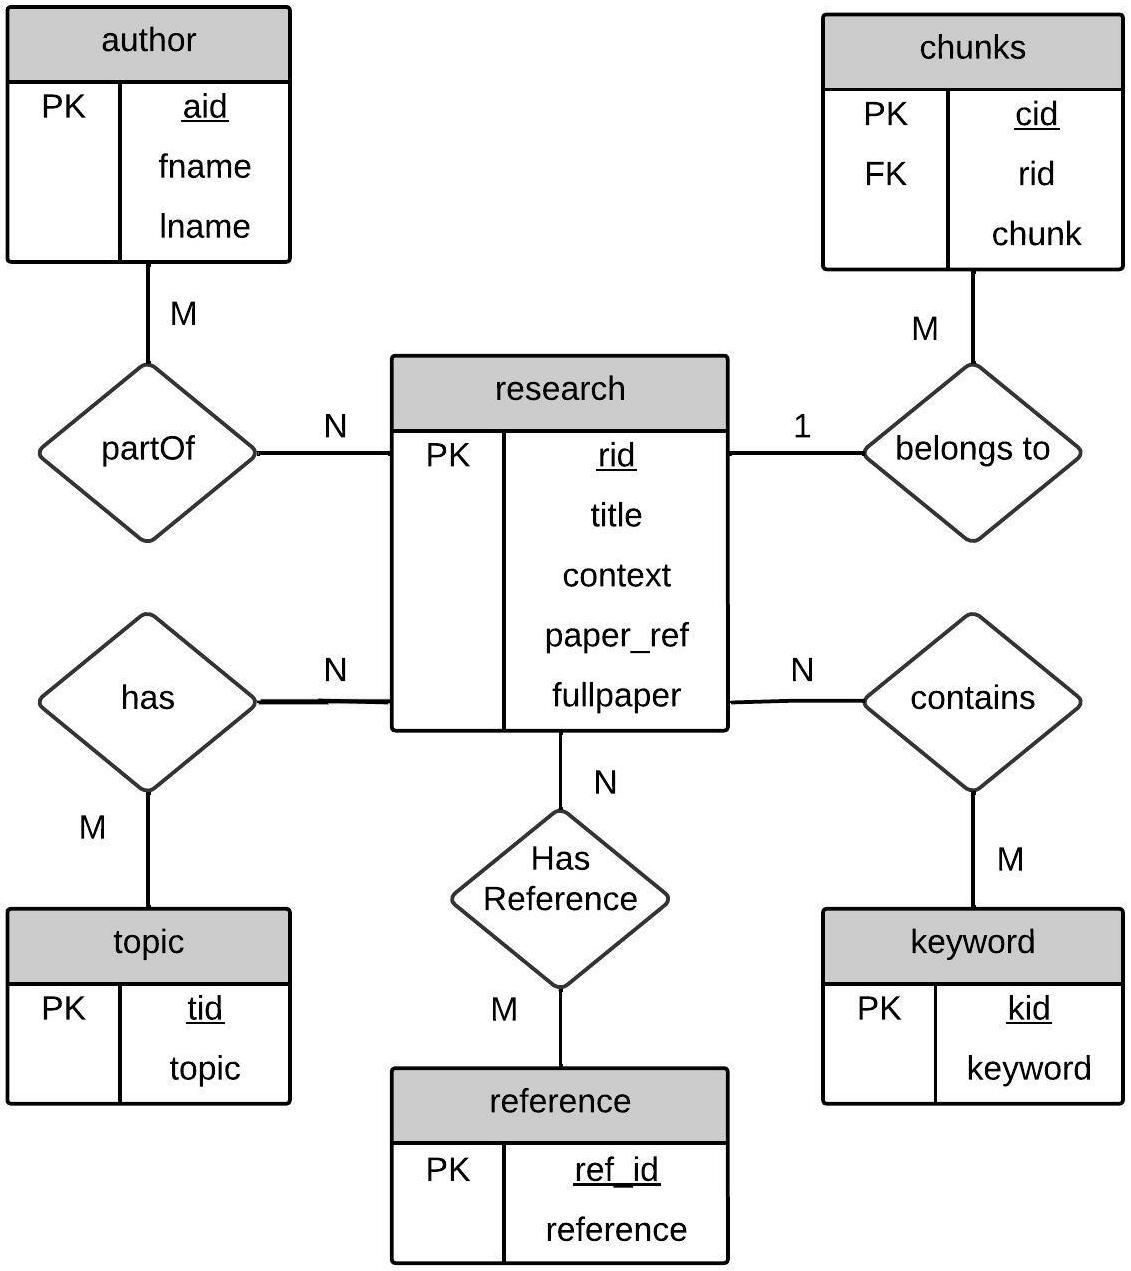
\includegraphics[width=0.42\textwidth]{figures/Table_diagram.jpeg} %specify width
	\end{center}
	\caption{Research Papers Schema Diagram} %specify caption
	\label{fig:table}
\end{figure}


We started the search with 85,000 peer-reviewed papers. After finishing the filtering and data cleaning, we ended with 56,365 different peer-reviewed papers. 


\subsection{Misinformation Rebuttal Pipeline}
After training the models and storing the context for the rebuttal, we create the model pipeline. The pipeline shown in Figure \ref{fig:llm} shows the process of receiving a text, making the classifications, and returning an explanation of why it is misinformation.

\begin{figure}[htbp]
	\begin{center}
		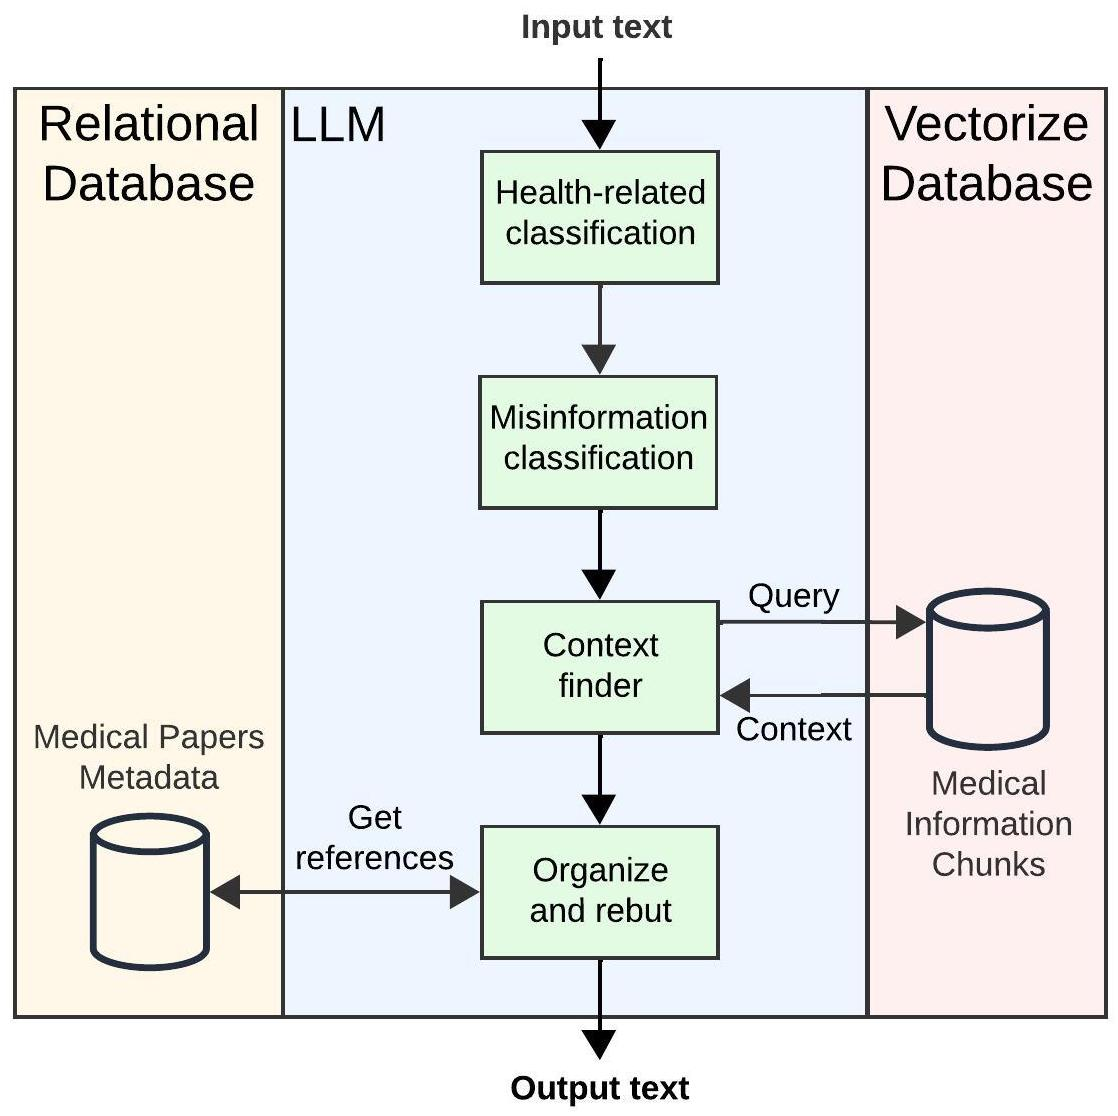
\includegraphics[width=0.42\textwidth]{figures/LLM_Pipeline.jpeg} %specify width
	\end{center}
	\caption{Misinformation Rebuttal Pipeline} %specify caption
	\label{fig:llm}
\end{figure}


\subsubsection{Health-related Classification}
The first part of the pipeline is determining if the text is related to health. If the text is related, we go to the next part of the pipeline. Non-related or ambiguous texts, ends the process because it is out of the model's scope. 

\subsubsection{Misinformation Classification}
Then, we validate if the input contains misinformation. The model can only return if the text misinformation or not. If the model finds no misinformation, the process is completed. When the result contains misinformation, we start the search for context for the rebuttal.

\subsubsection{Context Finder}
Before we the query the vector database, we must understand the topic of the text. To automate this process and generate a query as precise as possible, we use Ollama \cite{ollama}. We send a query to Ollama asking it to make a one-sentence query for the vector database related to the input.

{\footnotesize %
\begin{tcolorbox}[colback=gray!5,colframe=black!50,boxrule=0.4pt,arc=2pt,left=0.5mm,right=0.5mm,top=0.1mm,bottom=0.1mm,title=Example]
\textbf{Input:}  
``\#nih fauci, expected to be grilled tomorrow over ineffective \textit{...} universal \#influenza vax in 5, maybe 10 years?"

\vspace{0.25em}
\textbf{Output:}  
``Flu vaccine effectiveness and future universal influenza vaccination strategies."
\end{tcolorbox}
}
\indent The above example shows that Ollama can identify the topics of the original text. That output is sent to the Chroma database to retrieve the research papers' chunks. For this experiment, our model returns eight chunks. We selected
this number because it returns an appropriate amount of context without Ollama truncating the text. These chunks are then sent to another model to be analyzed and organized.

\subsubsection{Organize and Rebut}
The final part of our pipeline is using RAG to provide an answer that explains why the original text is misinformation. First, we retrieve the references of the chunks we use for the context. Then, we send the original text with the chunks, as context, to Ollama so the model can generate an explanation that rebuts the misinformation. The final output is a JSON with the classifications, a 2-3 sentence rebuttal generated by Ollama, and references used for the rebuttal.


The pipeline automates the classification process and rebut misinformation using peer-reviewed research. By leveraging fine-tuned models, vector search, and RAG, the architecture provides concise, fact-based responses. Also, this
approach has the ability to explain complex content accessible to non-technical readers. This can assist professionals in the field to mitigate the spread of lies that can negatively impact public health.


%\section{User Interface (UI)}
%With the pipeline correctly working, users need to interact and view the results. We created an user interface where they can interact with texts and see the classification process. Figure \ref{fig:Menu} shows the main menu of the interface. When we select a text, it triggers a side screen to appear that shows the results from the misinformation classification pipeline. 
%
%\begin{figure}[H]
%	\begin{center}
%		\frame{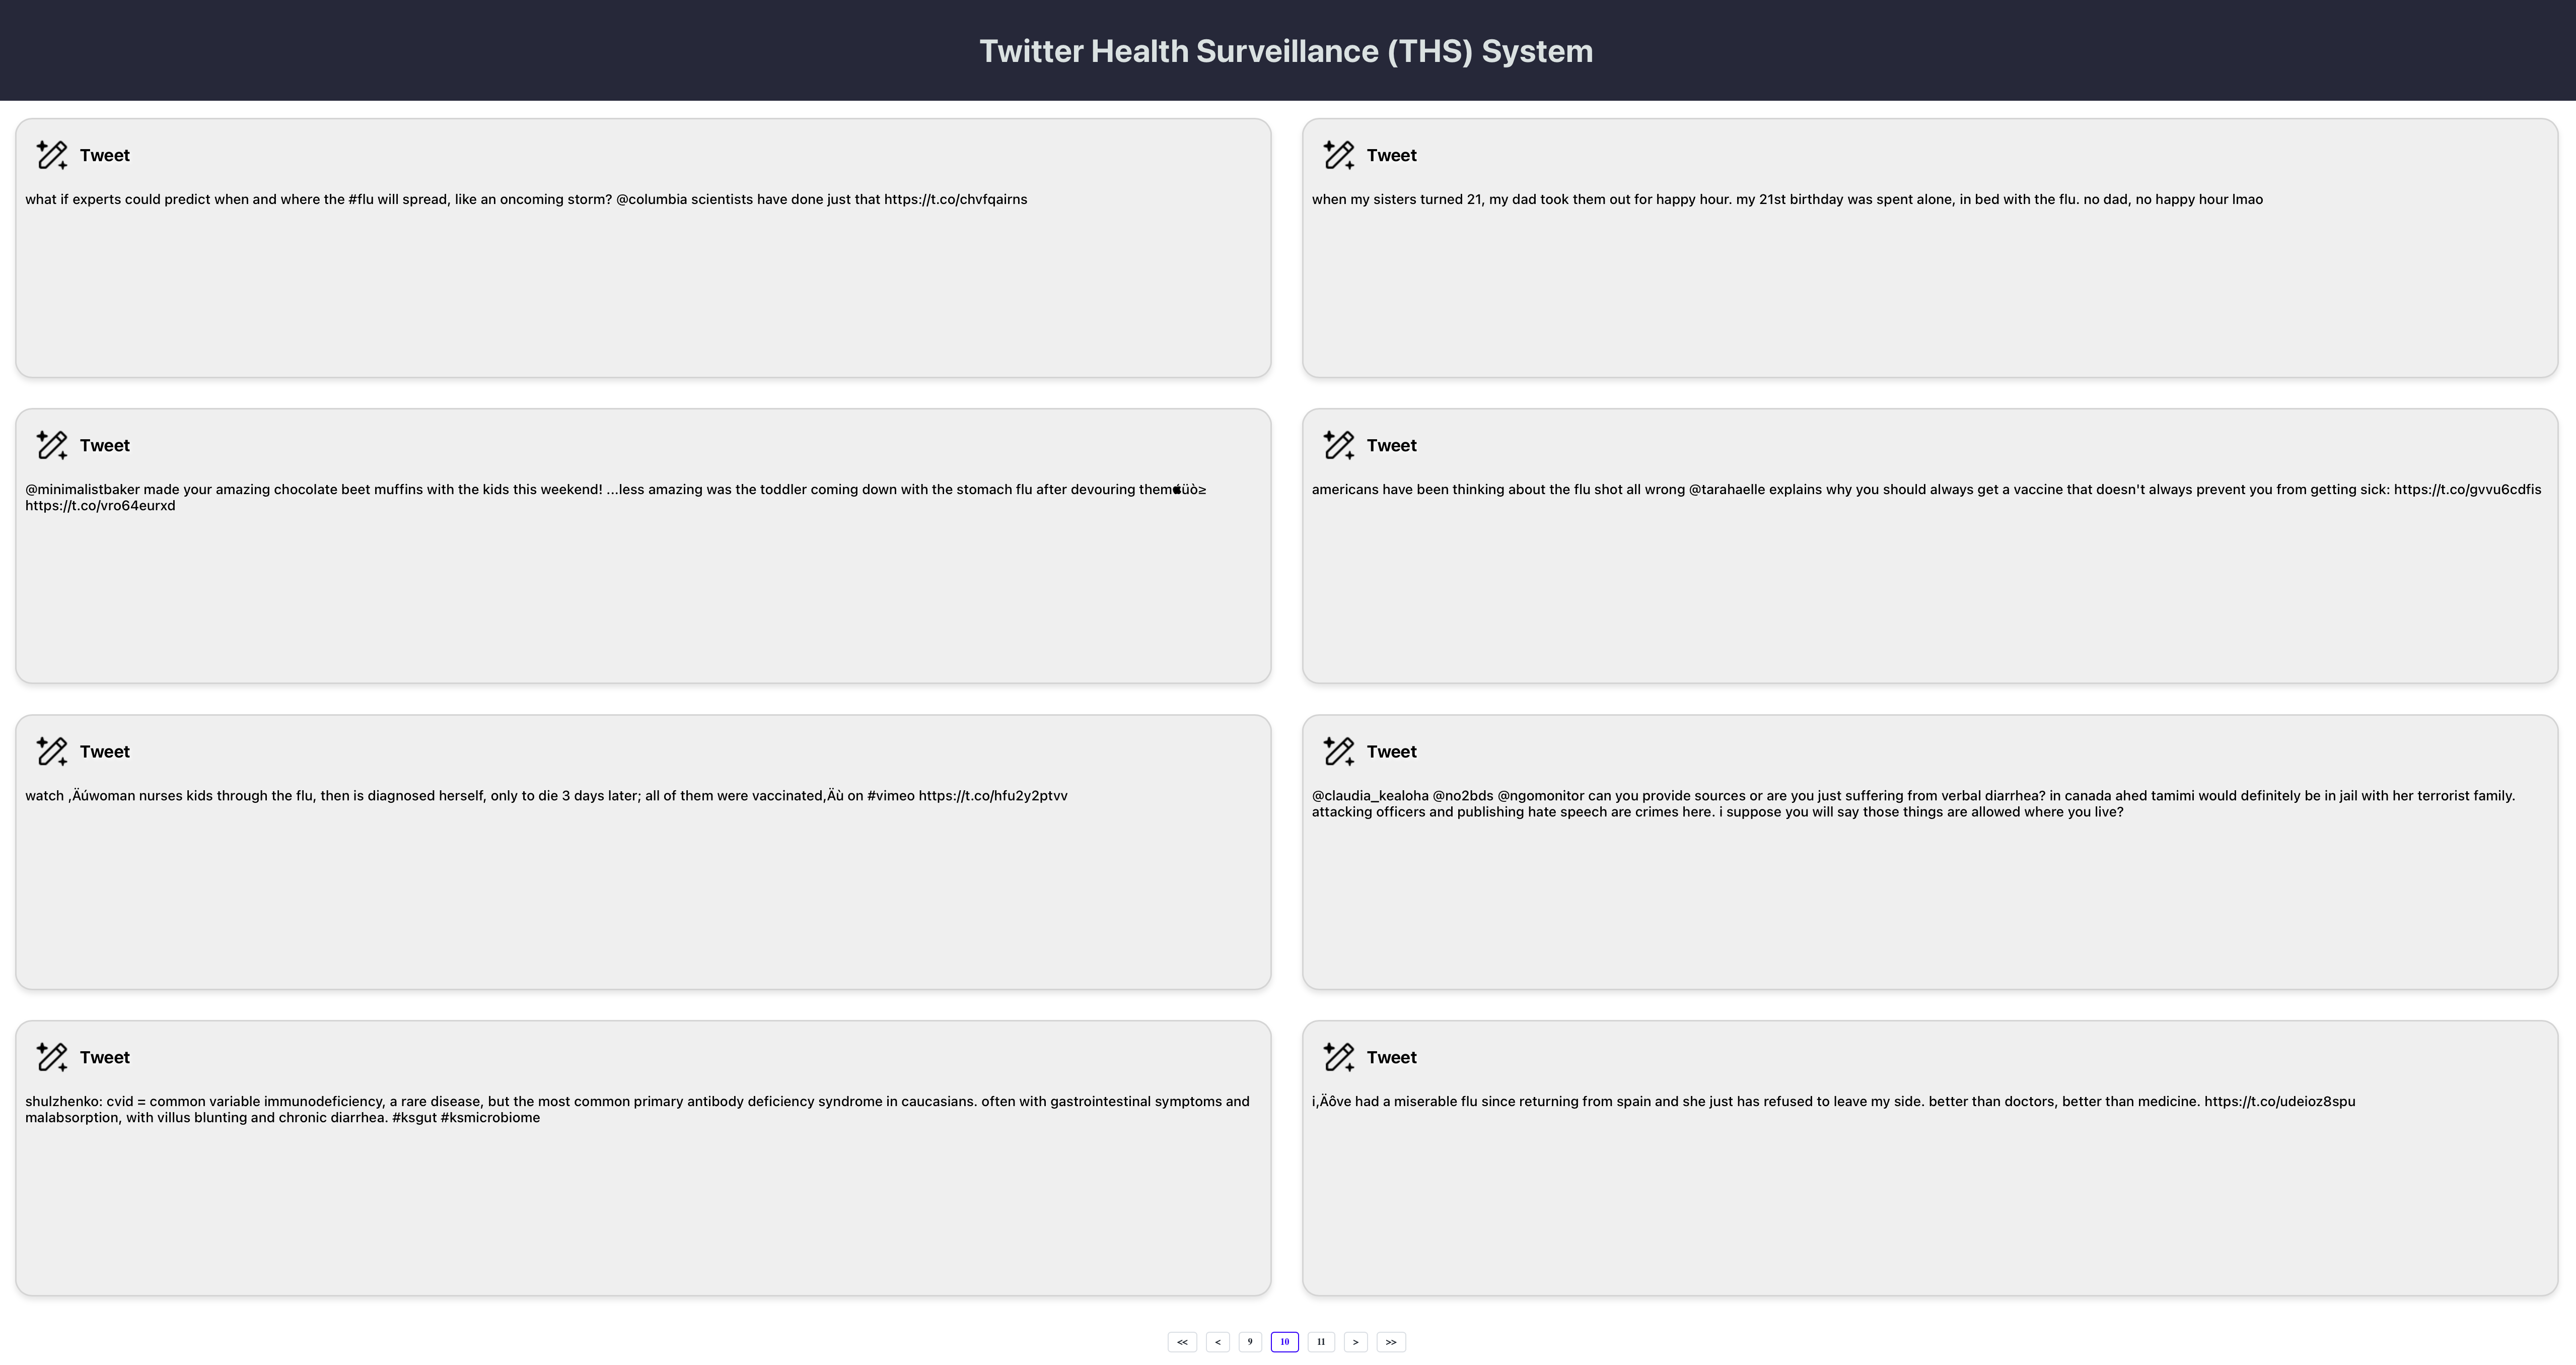
\includegraphics[width=0.67\paperwidth]{figures/THS_Frontend_Menu.png}} %specify width
%	\end{center}
%	\caption{THS Frontend - Menu} %specify caption
%	\label{fig:Menu}
%\end{figure}
%
%Figure \ref{fig:frontendmisinformation} presents a case where the models classified the text as health-related and misinformation. The side windows shows the original text, the classifications, and rebuttal. A clearer image of the side screen is shown in Figure \ref{fig:frontendrebuttal}. The top of the side screen shows the text that was classified. Number 1 shows the health classification, and number 2 shows the misinformation classification. Below that is the rebuttal generated by the models. Finally, we include the references of the research used for the rebuttal. 
%
%\begin{figure}[H]
%	\begin{center}
%		\frame{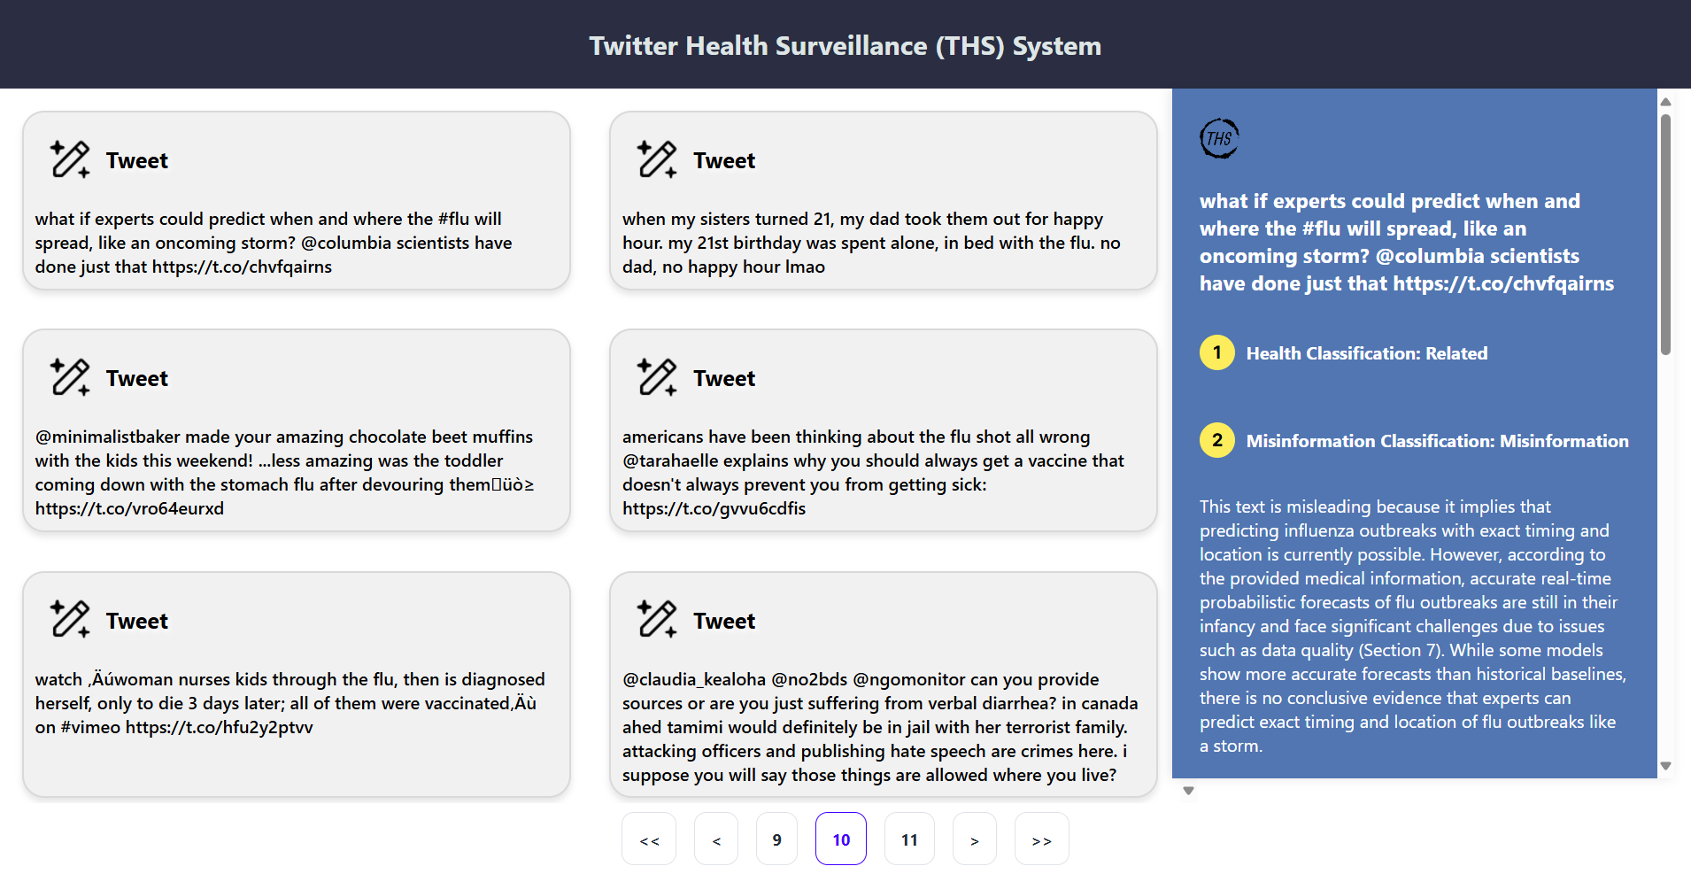
\includegraphics[width=0.67\paperwidth]{figures/THS_Misleading.png}} %specify width
%	\end{center}
%	\caption{THS Frontend - Misinformation Classification } %specify caption
%	\label{fig:frontendmisinformation}
%\end{figure}
%
%
%\begin{figure}[H]
%	\begin{center}
%		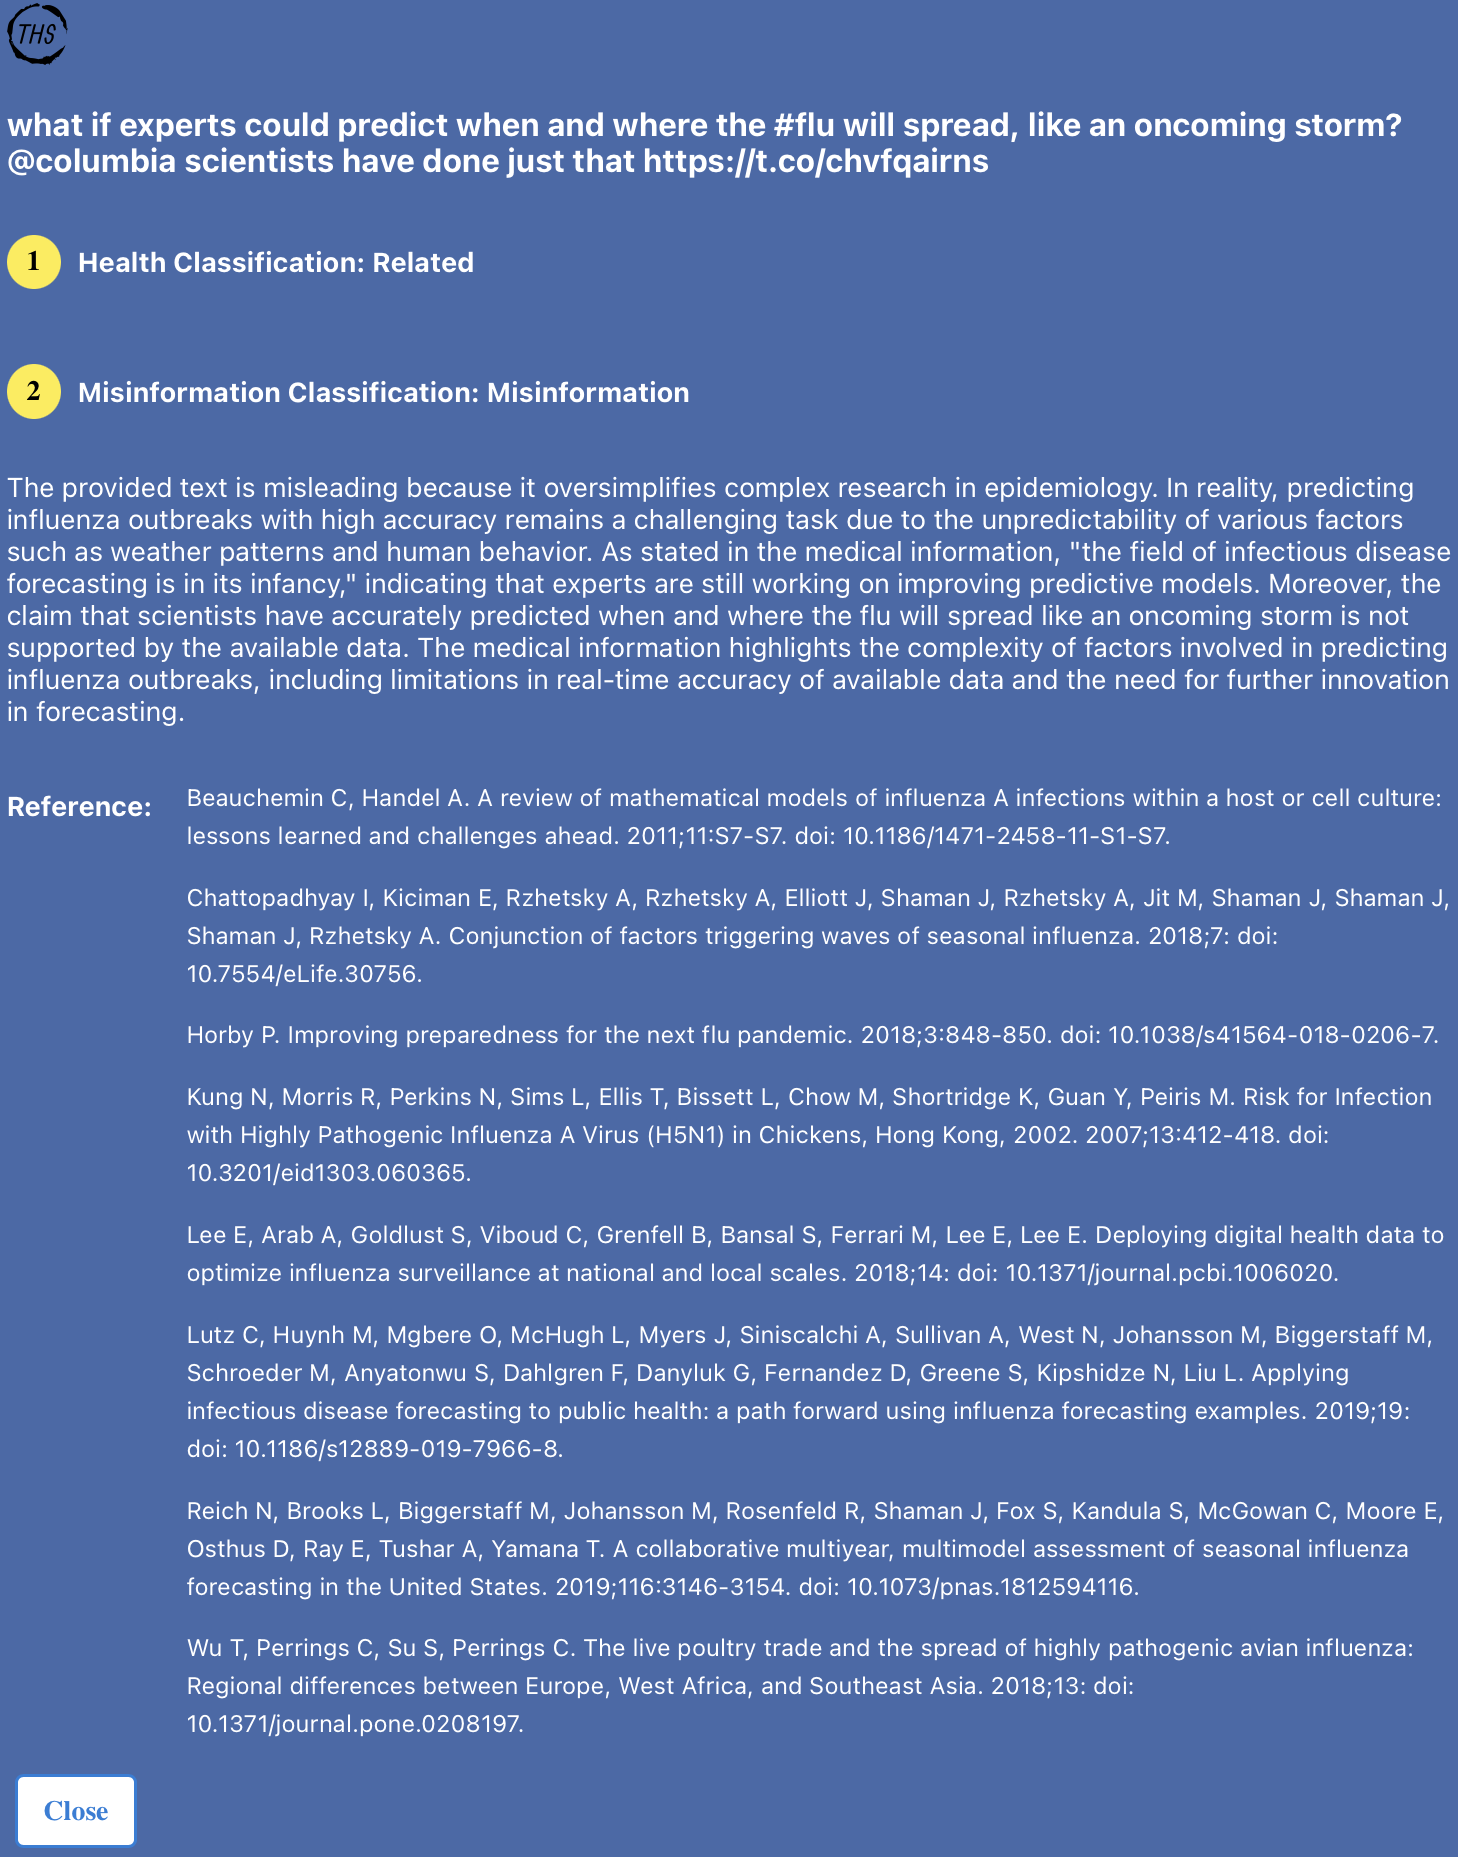
\includegraphics[width=0.75\textwidth]{figures/THS_Rebuttal_view.png} %specify width
%	\end{center}
%	\caption{THS Frontend  - Rebuttal View} %specify caption
%	\label{fig:frontendrebuttal}
%\end{figure}






